\documentclass[journal,12pt,twocolumn]{IEEEtran}

\usepackage{setspace}
\usepackage{gensymb}

\singlespacing


\usepackage[cmex10]{amsmath}

\usepackage{amsthm}

\usepackage{mathrsfs}
\usepackage{txfonts}
\usepackage{stfloats}
\usepackage{bm}
\usepackage{cite}
\usepackage{cases}
\usepackage{subfig}

\usepackage{longtable}
\usepackage{multirow}

\usepackage{enumitem}
\usepackage{mathtools}
\usepackage{steinmetz}
\usepackage{tikz}
\usepackage{circuitikz}
\usepackage{verbatim}
\usepackage{tfrupee}
\usepackage[breaklinks=true]{hyperref}
\usepackage{graphicx}
\usepackage{tkz-euclide}
\usepackage{float}

\usetikzlibrary{calc,math}
\usepackage{listings}
    \usepackage{color}                                            %%
    \usepackage{array}                                            %%
    \usepackage{longtable}                                        %%
    \usepackage{calc}                                             %%
    \usepackage{multirow}                                         %%
    \usepackage{hhline}                                           %%
    \usepackage{ifthen}                                           %%
    \usepackage{lscape}     
\usepackage{multicol}
\usepackage{chngcntr}

\DeclareMathOperator*{\Res}{Res}

\renewcommand\thesection{\arabic{section}}
\renewcommand\thesubsection{\thesection.\arabic{subsection}}
\renewcommand\thesubsubsection{\thesubsection.\arabic{subsubsection}}

\renewcommand\thesectiondis{\arabic{section}}
\renewcommand\thesubsectiondis{\thesectiondis.\arabic{subsection}}
\renewcommand\thesubsubsectiondis{\thesubsectiondis.\arabic{subsubsection}}


\hyphenation{op-tical net-works semi-conduc-tor}
\def\inputGnumericTable{}                                 %%

\lstset{
%language=C,
frame=single, 
breaklines=true,
columns=fullflexible
}
\begin{document}
\newtheorem{theorem}{Theorem}[section]
\newtheorem{problem}{Problem}
\newtheorem{proposition}{Proposition}[section]
\newtheorem{lemma}{Lemma}[section]
\newtheorem{corollary}[theorem]{Corollary}
\newtheorem{example}{Example}[section]
\newtheorem{definition}[problem]{Definition}

\newcommand{\BEQA}{\begin{eqnarray}}
\newcommand{\EEQA}{\end{eqnarray}}
\newcommand{\define}{\stackrel{\triangle}{=}}
\bibliographystyle{IEEEtran}
\providecommand{\mbf}{\mathbf}
\providecommand{\pr}[1]{\ensuremath{\Pr\left(#1\right)}}
\providecommand{\qfunc}[1]{\ensuremath{Q\left(#1\right)}}
\providecommand{\sbrak}[1]{\ensuremath{{}\left[#1\right]}}
\providecommand{\lsbrak}[1]{\ensuremath{{}\left[#1\right.}}
\providecommand{\rsbrak}[1]{\ensuremath{{}\left.#1\right]}}
\providecommand{\brak}[1]{\ensuremath{\left(#1\right)}}
\providecommand{\lbrak}[1]{\ensuremath{\left(#1\right.}}
\providecommand{\rbrak}[1]{\ensuremath{\left.#1\right)}}
\providecommand{\cbrak}[1]{\ensuremath{\left\{#1\right\}}}
\providecommand{\lcbrak}[1]{\ensuremath{\left\{#1\right.}}
\providecommand{\rcbrak}[1]{\ensuremath{\left.#1\right\}}}
\theoremstyle{remark}
\newtheorem{rem}{Remark}
\newtheorem*{remark}{Remark}
\newcommand{\sgn}{\mathop{\mathrm{sgn}}}
\providecommand{\abs}[1]{\vert#1\vert}
\providecommand{\res}[1]{\Res\displaylimits_{#1}} 
\providecommand{\norm}[1]{\lVert#1\rVert}
%\providecommand{\norm}[1]{\lVert#1\rVert}
\providecommand{\mtx}[1]{\mathbf{#1}}
\providecommand{\mean}[1]{E[ #1 ]}
\providecommand{\fourier}{\overset{\mathcal{F}}{ \rightleftharpoons}}
%\providecommand{\hilbert}{\overset{\mathcal{H}}{ \rightleftharpoons}}
\providecommand{\ztrans}{\overset{\mathcal{Z}}{ \rightleftharpoons}}
\providecommand{\system}{\overset{\mathcal{H}}{ \longleftrightarrow}}
	%\newcommand{\solution}[2]{\textbf{Solution:}{#1}}
\newcommand{\solution}{\noindent \textbf{Solution: }}
\newcommand{\cosec}{\,\text{cosec}\,}
\providecommand{\dec}[2]{\ensuremath{\overset{#1}{\underset{#2}{\gtrless}}}}
\newcommand{\myvec}[1]{\ensuremath{\begin{pmatrix}#1\end{pmatrix}}}
\newcommand{\mydet}[1]{\ensuremath{\begin{vmatrix}#1\end{vmatrix}}}
\numberwithin{equation}{subsection}
\makeatletter
\@addtoreset{figure}{problem}
\makeatother
\let\StandardTheFigure\thefigure
\let\vec\mathbf
\renewcommand{\thefigure}{\theproblem}
\def\putbox#1#2#3{\makebox[0in][l]{\makebox[#1][l]{}\raisebox{\baselineskip}[0in][0in]{\raisebox{#2}[0in][0in]{#3}}}}
     \def\rightbox#1{\makebox[0in][r]{#1}}
     \def\centbox#1{\makebox[0in]{#1}}
     \def\topbox#1{\raisebox{-\baselineskip}[0in][0in]{#1}}
     \def\midbox#1{\raisebox{-0.5\baselineskip}[0in][0in]{#1}}
\vspace{3cm}
\title{GATE ASSIGNMENT 1}
\author{Vojeswitha Gopireddy \\ AI20BTECH11024}
\maketitle
\newpage
\bigskip
\renewcommand{\thefigure}{\theenumi}
\renewcommand{\thetable}{\theenumi}
Download all python codes from 
\begin{lstlisting}
https://github.com/V-Gopireddy/EE3900/blob/main/GATE_Assignment1/codes/GATE_Assignment-1.py
\end{lstlisting}
%
and latex-tikz codes from 
%
\begin{lstlisting}
https://github.com/V-Gopireddy/EE3900/blob/main/GATE_Assignment1/GATE_Assignment-1.tex
\end{lstlisting}
%
\section{GATE EC 2017 Q.35}
Consider the parallel combination of two LTI systems shown in the figure.

\begin{figure}[h]
    \centering
    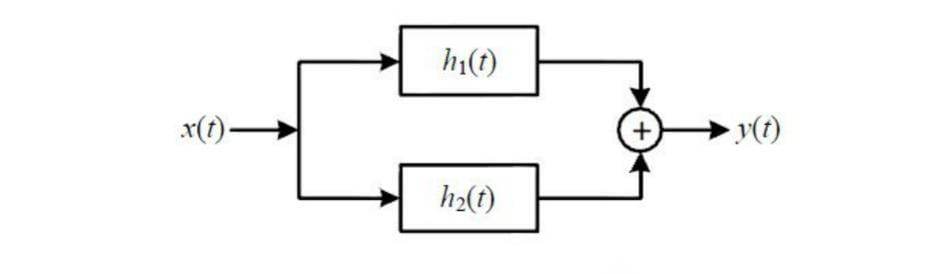
\includegraphics[width=\columnwidth]{LTI-systems.jpeg}
    %\caption{Parallel combination of two LTI systems}%
    \label{fig:my_label}
\end{figure}

The impulse responses of the systems are
\begin{align}
    h_1(t) &= 2\delta(t+2) - 3\delta(t+1)\\
    h_2(t) &= \delta(t-2)
\end{align}
If the input $x(t)$ is a unit step signal, then find the energy of $y(t)$. 
%
\section{Solution}
\begin{theorem}[Convolution Theorem] \label{ct}
Let $F(z)$ and $G(z)$ be the Z-transform of two functions $f$ and $g$ respectively. Then
\begin{align}
\mathcal{Z}(f * g)=F(z)G(z)
\end{align}
\end{theorem}
\begin{lemma}
Let $u(t)$ be unit step funtion and $\delta(t)$ be dirac-delta function. Then for any real number c,
\begin{align}
    u(t)*\delta(t-c) = u(t-c)\label{eqn}
\end{align}
\end{lemma}
\begin{proof}
We know,
\begin{align}
    \delta(t) \ztrans 1\\
    \implies {\mathcal{Z}}\{\delta(t-c)\} &= z^{-c}{\mathcal{Z}}\{\delta(t)\} = z^{-c}
\end{align}
And
\begin{align}
U(z) = \frac{1}{1-z^{-1}}, \quad \abs{z} > 1
\end{align}
We have,
\begin{align}
\mathcal{Z}\cbrak{u(t)*\delta(t-c)} &= \mathcal{Z}\cbrak{\delta(t-c)}U(z)\\ &= \frac{z^{-c}}{1-z^{-1}}\\ &= z^{-c}\sum _{n=0 }^{\infty}z^n\\ &= \mathcal{Z}\cbrak{u(t-c)}\\
\implies u(t)*\delta(t-c) &= u(t-c) 
\end{align}
\end{proof}
Given that,
\begin{align}
    h_1(t) &= 2\delta(t+2) - 3\delta(t+1)\\
    h_2(t) &= \delta(t-2)
\end{align}
Overall impulse response of the system is,
\begin{align}
    h(t) &= h_1(t) + h_2(t)\\  &= 2\delta(t+2) - 3\delta(t+1) + \delta(t-2)
\end{align}
Given input, $x(t) = u(t)$, then output signal $y(t)$ is given by,
\begin{align}
    y(t) &= x(t)*h(t)\\ 
    &= u(t)*[2\delta(t+2) - 3\delta(t+1) + \delta(t-2)]
\end{align}
From \eqref{eqn} we have,
\begin{align}
    y(t) &= 2u(t+2) -3u(t+1) + u(t-2) 
\end{align}
Solving we get,
\begin{align}
      y(t) &= 
     \begin{cases}
    2, & -2 \leq t < -1 \\~\\[-1em]
	-1, & -1 \leq t < 2 \\~\\[-1em]
	0, & \text{otherwise}
	\end{cases}
\end{align}
Energy of the output signal $E_y$ is given by,
\begin{align}
    E_y &= \int_{-\infty}^{\infty}\abs{y(t)}^2dt\\
    &= \int_{-2}^{-1}4dt + \int_{-1}^{2}dt\\
    &= 7
\end{align}
\begin{figure}[h!]
\centering
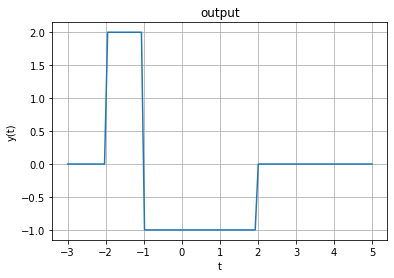
\includegraphics[width=\columnwidth]{Output-signal.png}
\caption{Output signal $y(t)$}
\label{fig:ellipse}
\end{figure}
\end{document}